\documentclass[legalpaper]{article}
\usepackage[legalpaper, margin=1in]{geometry}
\usepackage[T1]{fontenc}
\usepackage[utf8]{inputenc}
\usepackage[italian]{babel}
\usepackage{graphicx}
\usepackage[table,xcdraw]{xcolor}
\usepackage{tabularx}
\usepackage{Cormorant Garamond}
\usepackage{titling}
\newcommand{\subtitle}[1]{%
	\posttitle{%
		\par\end{center}
	\begin{center}\large#1\end{center}
	\vskip0.5em}%
}
\usepackage[linktocpage=true]{hyperref}



\begin{document}
\title{\textbf{PROGETTO BASI DI DATI}} \large
\subtitle{Progettazione ed implementazione di una base di dati relazionale per la gestione delle assistenze di una ditta di gestione di impianti di riscaldamento.}
\author{\textit{Parata Loris 144338} \and \textit{Brugnera Matteo 137370} \and \textit{Rasera Giovanni 143395}}
\maketitle
\begin{figure}[ht]
	\centering
	
\includegraphics[width=10cm]{image/Udine}
	\label{Udine}
\end{figure}

\textbf{Contatti:}
\begin{itemize}
	\item \textit{144338@spes.uniud.it}
	\item \textit{137370@spes.uniud.it}
	\item \textit{143395@spes.uniud.it}
\end{itemize}
\textbf{Link utili:}
\begin{itemize}
	\item Github: \href{https://github.com/GiovanniRaseraF/ProgettoBasiDiDatiLaboratorio}{https://github.com/GiovanniRaseraF/ProgettoBasiDiDatiLaboratorio}
\end{itemize}
\newpage


\tableofcontents

\newpage
\section{Introduzione}
\rule{\linewidth}{1.5pt}
\subsection{Introduzione}
Lo scopo del progetto è quello di implementare un \textbf{sistema informativo}, nello specifico una base di dati relazionale, in grado di \textbf{gestire le prestazioni di un centro di assistenza per impianti di riscaldamento}.\\ \newline
Le funzionalità che dovrà prevedere il sistema sono di seguito specificate.\\
L'azienda deve permettere di gestire le \textbf{richieste di assistenza}, che sono a loro volta \textbf{composte da un insieme di interventi effettuati da tecnici specializzati}.\\
I servizi offerti sono usufruibili solo da \textbf{clienti facenti parte di due tipologie} di \textbf{persone giuridiche}, che rappresentano \textbf{aziende} ed \textbf{enti pubblici}, oppure da persone fisiche che rappresentano i \textbf{singoli cittadini}.
Ognuno di essi avrà un \textbf{codice identificativo} generato dal sistema una volta divenuti clienti, grazie al quale si potrà risalire a tutti i loro dati.
In particolare, per le aziende e gli enti pubblici si vuole tenere il codice di Partita IVA, mentre per i singoli cittadini il Codice Fiscale.\\
Le assistenze vengono identificate univocamente dal \textbf{codice di Richiesta d'Assistenza}. Ogni intervento è legato all'assistenza ed identificato univocamente da un \textbf{numero progressivo}. 
Le richieste di assistenza vengono accettate solamente se la tipologia del problema è presente nella lista di problematiche risolvibili. \\ \newline
Per ogni intervento, si tiene traccia di:
\medskip
\begin{itemize}
    \item \textbf{cliente} richiedente l'assistenza;
    \item \textbf{tipologia} del \textbf{guasto};
    \item \textbf{seriale} del sistema di riferimento;
    \item \textbf{tecnico} assegnato;
    \item \textbf{codice} identificativo \textbf{dell'intervento};
    \item \textbf{modalità d'intervento};
    \item \textbf{data} intervento;
    \item \textbf{durata} intervento.
\end{itemize}


\newpage
\section{Raccolta e analisi dei requisiti}
\rule{\linewidth}{1.5pt}
\subsection{Tabella dei requisiti}
Questa fase rappresenta l’\textbf{inizio della realizzazione} di un sistema informativo.
Con essa si cerca di \textbf{comprendere quali sono gli obiettivi} che vengono richiesti.\\ 
È necessario \textbf{porre} particolare \textbf{attenzione alla terminologia utilizzata}, in modo tale da poter procedere alla formulazione dei requisiti.

\subsection{Glossario dei termini}
Il linguaggio naturale è ambiguo, ecco perché è necessario chiarire con precisione ogni termine utilizzato durante questa fase di progettazione.\\
Per ogni termine introdotto si definiscono:
\begin{itemize}
    \item \textbf{Descrizione}: definizione semantica del termine
    \item \textbf{Sinonimi}: eventuali sinonimi utilizzati per identificare lo stesso oggetto
    \item \textbf{Correlazioni}: le relazioni esistenti tra i diversi oggetti
\end{itemize}
\medskip
Il seguente glossario definisce i termini più rilevanti che saranno l’input della fase di progettazione concettuale.\\ \newline
\medskip
\renewcommand\arraystretch{1,5}
\begin{tabular}{ |p{1.8cm}|p{8cm}|p{3cm}|p{2.5cm}| }
\hline
\multicolumn{4}{|c|}{\textbf{Glossario}} \\
\hline
\textbf{Termine} & \textbf{Descrizione} & \textbf{Sinonimo} & \textbf{Correlazione} \\
\hline
\textit{Cliente} &  soggetto che effettua una richiesta di assistenza all'azienda di assistenza & Persona Giuridica \newline Persona fisica & Assistenza\\
\hline

\textit{Persona \newline fisica} &  soggetto che rappresenta se stesso e che effettuerà una richiesta di assistenza &  Singolo cittadino \newline Cliente &  Cliente \\ \hline

\textit{Persona \newline giuridica} &  persona fisica che rappresenta un'azienda o un ente pubblico che effettuerà una richiesta di assistenza & Azienda \newline Ente Pubblico \newline Cliente &  Cliente \\ \hline

\textit{Richiesta d'assistenza} & inizializzazione di un nuovo contratto di assistenza tra un cliente e l'azienda di assistenza, ogni richiesta d'assistenza composta è da almeno un intervento   & Non ha sinonimi & Cliente \newline Intervento \newline Tip. di guasto \\ \hline

\textit{Intervento} & prestazione eseguita da un tecnico per risolvere un guasto & Prestazione & Tip. di guasto \newline Tecnico \\ \hline

\textit{Tecnico}  & dipendente dell'azienda di assistenza, specializzato nella risoluzione di varie tipologie di guasto & Dipendente & Tip. guasto \newline Intervento \\ \hline

\textit{Tipologia di guasto}  & problematica specifica da risolvere  & Problema &  Tecnico  \newline Cliente \newline Assistenza \\ \hline

\end{tabular}
\pagebreak

\subsection{Riscrittura dei requisiti}
In questa fase vengono \textbf{tradotte le richieste della consegna in requisiti da soddisfare} e viene definito il ruolo delle entità all'interno della base di dati.\\
\newline
\renewcommand\arraystretch{1,5}
\begin{tabular}{ |p{16 cm}| }
\hline
\multicolumn{1}{|c|}{\textbf{Riscrittura dei requisiti}} \\
\hline
\textbf{Frasi di natura generale}  \\
\hline
- Si vuole implementare un sistema automatico per la gestione dei servizi di assistenza e dei relativi interventi di un'azienda d'assistenza di impianti di riscaldamento \newline
- Le assistenze possono essere richieste solamente per problemi risolvibili dai tecnici dell'azienda.\\ \hline
\textbf{Frasi relative al cliente}  \\
\hline
-  I clienti possono essere di diversa natura:\newline
- Persona Giuridica, che a sua volta può essere un'azienda oppure un ente pubblico; \newline
- Singolo cittadino, ovvero persona fisica; \newline
- I clienti richiedono un'assistenza relativa ad una specifica tipologia di guasto, specificandone il seriale del sistema di riferimento .\newline
- I clienti sono identificati univocamente dal proprio codice fiscale o partita Iva, in base alla tipologia del cliente e dai relativi dati anagrafici del cliente stesso o del referente aziendale, un recapito telefonico, un indirizzo e la città in cui risiede.\\
\hline
\textbf{Frasi relative alla richiesta d'assistenza}  \\
\hline
- Un'assistenza è caratterizzata da un codice identificativo generato dal sistema. Nel momento in cui viene completata l'assistenza viene memorizzata la data dell'ultimo intervento.\\
\hline
\textbf{Frasi relative all'intervento}  \\
\hline
- Un intervento è caratterizzato da :\newline 
- un numero progressivo, che fa riferimento alla richiesta d'assistenza a cui appartiene: \newline
- modalità con la quale può essere eseguito (da remoto o in sede)\newline
- dalla data e dalla relativa durata del singolo intervento misurato in ore (0-24). \newline 
- Un solo intervento può essere eseguito durante l'arco della giornata lavorativa.\\
\hline
\textbf{Frasi relative al tecnico}  \\
\hline
- Un tecnico è identificato dal suo codice fiscale, dai suoi dati anagrafici, un recapito telefonico, una data di assunzione e indirizzo del domicilio.\newline
-Inoltre sarà presente il conteggio mensile delle ore lavorate.
\\
\hline
\textbf{Frasi relative al guasto}  \\
\hline
- Una tipologia di guasto è rappresentata da: \newline
- codice univoco, \newline
- descrizione del problema.\\
\hline
\textbf{Frasi relative al coinvolgimento di cliente, assistenza e tipologia guasto}  \\
\hline
- Quando un cliente richiede un'assistenza relativa ad uno specifico guasto, per poter finalizzare e registrare la data di inizio assistenza è necessario che sia presente quella tipologia di guasto tra i guasti riparabili e l'inserimento del numero seriale del sistema di riferimento.\\
\hline
\textbf{Frasi relative al coinvolgimento di tecnico e tipologia guasto}  \\
\hline
- Un tecnico può essere assunto se è capace di risolvere almeno una tipologia di guasto , ma nel tempo può ampliare le proprie competenze e risolvere problemi anche di tipologia diversa.\\
\hline

\textbf{Frasi relative al coinvolgimento di assistenza, intervento, tecnico e tipologia guasto}  \\
\hline
- Una volta effettuata la richiesta di assistenza, si pianifica il primo intervento assegnando un tecnico competente per risolvere quella tipologia di guasto, controllando che in quella data non ci sia un intervento programmato per lo stesso tecnico altrove.\\
\hline
\end{tabular}
\newpage

\subsection{Caso di studio} 
	Per la realizzazione del sistema informativo è stato \textit{teorizzato un business-plan} di un'azienda di piccole/medie dimensioni che opera a livello regionale.
	Consideriamo la seguente situazione dopo 10 anni di attività:
	\begin{itemize}
		\item numero \textbf{clienti totale}: 10.000 (fedeli e non) \footnote[1]{\textbf{per fedeli si intende tutti quei clienti che faranno rifermento a noi come aziende per qualsiasi guasto negli anni a venire}};
		\item numero \textbf{tecnici totali}: 75;
		\item media \textbf{clienti annuali}: 10.00;
		\item \textbf{media di 2 richieste di assistenza} per cliente all'anno;
		\item \textbf{media di 3 interventi per ogni assistenza} richiesta;
		\item in \textbf{media 300 clienti rimangono fedeli} al nostro servizio;
	\end{itemize}
	Supponiamo che dei 10.000 clienti avuti in 10 anni, 300 siano rimasti fedeli a noi. Di conseguenza l'undicesimo anno operativo dell'azienda otterrà 3.000+1.000=4.000 clienti (fedeli + nuovi clienti annuali, fedeli e non). Facendo così, avremo 4.000*2=8.000 assistenze totali e quindi 24.000 interventi.\\
	Quest'ultimi vengono divisi tra i 75 tecnici, facendo sì che ognuno di essi abbia in media 320 interventi da eseguire in un anno.\\
	Nel dodicesimo anno otteniamo un totale di 3.300 clienti fedeli, arrivando a fine anno con 4.300 clienti e 25.800 interventi fatti, ovvero 344 a tecnico. Tutto ciò risulta essere troppo oppressivo per un lavoratore, quindi dobbiamo aumentare il numero di tecnici da assumere a fronte dell'aumento della clientela, aumentando così il volume dell'azienda stessa.\\
	Se supponiamo che ogni anno vengono assunti e/o formati 6 nuovi dipendenti, abbiamo che il rapporto interventi/tecnici rimane sempre intorno ai 320 (ovvero ogni tecnico avrà 320 interventi all'anno).\\
	Ad esempio il tredicesimo anno avremmo 87 operai con 27.600 interventi, cioè intorno ai 317 interventi per operaio.\\
	Ultimo appunto importante riguarda la distinzione che è possibile fare tra i vari clienti.
	Più in particolare del 100\% dei clienti, il 50\% risulta essere un ente pubblico mentre il restante 50\% è privato. Del 50\% pubblico, il suo 70\% fa riferimento alle aziende, mentre il 30\% agli enti pubblici.
	
	\subsection{Requisiti operazionali}
	Le \textbf{operazioni principali} che prenderemo in considerazione sono:
	\begin{itemize}
		\item \textbf{operazione 1}: date le informazioni di un nuovo cliente, inserirlo nella base di dati --> \textit{19 volte a settimana};
		\item \textbf{operazione 2}: date le informazioni necessarie fornite da un cliente, aggiungere una richiesta d'assistenza relativa ad una tipologia di problema --> \textit{150 volte a settimana};
		\item \textbf{operazione 3}: data l'informazione di una richiesta d'assistenza, creare un nuovo intervento relativo ad essa --> \textit{450 volte a settimana};
		\begin{itemize}
			\item \textbf{operazione 3.1}: Ricerca e classificazione in base al numero di interventi eseguiti nel mese corrente dei tecnici capaci di risolvere la tipologia di guasto presente nella richiesta di assistenza.
			\item \textbf{operazione 3.2}: Assegnazione del tecnico all'intervento.
			\item \textbf{operazione 3.3}: Creazione dell'intervento.
		\end{itemize}
		\item \textbf{operazione 4}: date le informazioni di un nuovo dipendente e delle tipologie di gusti che è capace di risolvere, aggiungerlo alla base di dati --> \textit{6 all'anno};
		\item \textbf{operazione 5}: dato il codice identificativo del cliente, visualizzare le relative richieste d'assistenza effettuate --> \textit{30 a settimana};
		\item \textbf{operazione 6}: visualizzare il numero di ore mensili di lavoro effettuate da ogni tecnico --> \textit{26 al mese};
		\item \textbf{operazione 7}: dato la tipologia di guasto, il numero di interventi eseguiti su di esso, ed i tecnici specializzati su quella tipologia, visualizzare per ogni tipologia guasto la relativa percentuale di forza lavoro disponibile a risolverla.  --> \textit{1 volta all'anno}. \\ Questo dato può essere utilizzato per vedere in quali reparti ci sono carenze di tecnici, andando così a mirare l'assunzione/training dei nuovi dipendenti;
		\item \textbf{operazione 8}: dato il codice identificativo di una richiesta di assistenza, visualizzare lo storico degli interventi --> \textit{10 volte al giorno}. \\Si vuole monitorare il più possibile l'impiego dei tecnici, cioè chi è impegnato e dove;
		\item \textbf{operazione 9}: dato il codice identificativo di un cliente ed una data, visualizzare il tempo complessivo degli interventi effettuati da quel momento --> \textit{1 volta a settimana};
		
	\end{itemize}


\newpage
\section{Progettazione concettuale}
\rule{\linewidth}{1.5pt}

\subsection{Definizione specifiche}
Per scrivere il nostro schema e per descrivere le specifiche e realizzare la relazione abbiamo utilizzato questa convenzione:
\begin{itemize}
	\item Entità: prima lettera MAIUSCOLA e il resto minuscolo\\
	Esempio: Assistenza, Cliente, Intervento.
	\item Relazione: tutta la parola minuscola\\
	Esempio: è capace di risolvere, composta da.
	\item Attibuti delle entità e delle relazioni: prima lettera minuscola e il resto della parola cammellizzato\\
	Esempio: dataFineAssistenza, numeroIntervento, dataAssunzione.
	\item Rappresentazione di un attributo di un entità o di una relazione: utilizzato il simbolo      ->      tra l'entità e l'attributo\\
	Esempio: Entità->attributoUno, Entità->attributoDue, Intervento->modalità.
\end{itemize}

\subsection{Schema Entità-Relazione}
Il modello Entità-Relazione (E-R) è il modello teorico utilizzato in questa fase di progettazione concettuale per la rappresentazione grafica e concettuale dello scenario di interesse. Questo permette di comprendere in modo semplice ed intuitivo quali sono i soggetti principali della scena e come sono relazionati tra di loro. 
Modello E-R dell'azienda di assistenza:
\newline

\begin{figure}[ht]
	\centering
	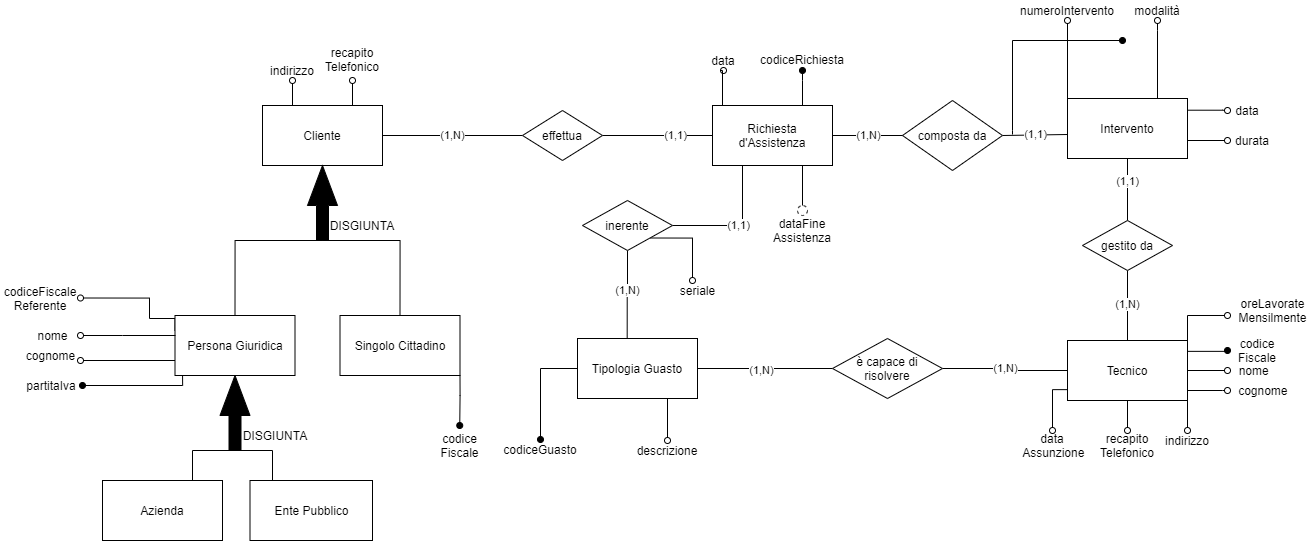
\includegraphics[width=1.1\linewidth]{image/schema_er.png}
	\caption[]{Schema E/R complessivo}
	\label{fig:erprototipov2}
\end{figure}


\subsubsection{Evidenziazione dello schema E-R}



\begin{figure}[!ht]
	\centering
	\begin{minipage}[b]{0.8\textwidth}
		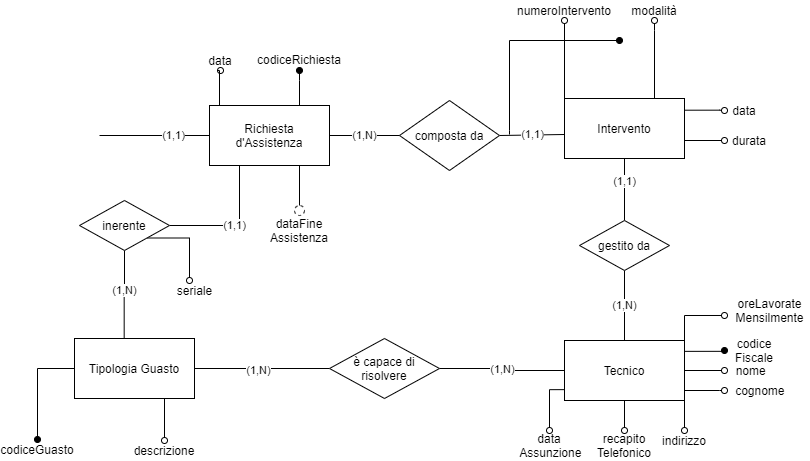
\includegraphics[width=\linewidth]{image/ciclo.png}
			\caption{Ciclo}
		\label{fig:ciclo}

	\end{minipage}
\hfill

\end{figure}

\paragraph{Figura 2}
in questa porzione di schema ER troviamo un ciclo. Esso è composto dalle seguenti Entità: 
		\begin{itemize}
			\item Richiesta d'Assistenza;
			\item Intervento;
			\item Tecnico;
			\item Tipologia Guasto;
		\end{itemize}
		
		Intervento è relazionato a Tecnico tramite \textit{"gestito da"}, una relazione \textbf{uno a molti}. Infatti, un Intervento è gestito da un singolo Tecnico in giornata, mentre un Tecnico può gestire uno o più Interventi.\\	
		Quest'ultimo però può risolvere solo un numero finito di tipologie di problemi, descritti dalla relazione \textbf{molti a molti} \textit{"è capace di risolvere"}, dove un Tecnico è in grado di risolvere più problemi, ed essi possono essere risolti da più Tecnici.\\
		Quest'ultimo fa sì che il ciclo non sia problematico perché un Tecnico che non ha le conoscenze per riparare un Guasto non può farlo.\\
		Infine, la Tipologia Guasto è legato con Richiesta d'Assistenza tramite la relazione \textbf{uno a molti} \textit{"inerente"}, dove una Tipologia Guasto può essere inerente a più Richieste d'Assistenza, mentre una Richiesta fa riferimento ad una sola Tipologia di Guasto.

\begin{figure}
		\centering
		\begin{minipage}[b]{0.4\textwidth}
			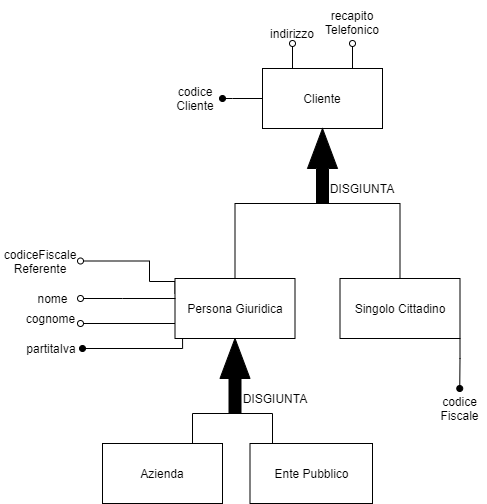
\includegraphics[width=\linewidth]{image/generalizzazione.png}
				\caption{Generalizzazione}
			\label{fig:generalizzazione}
	\end{minipage}
	\hfill
	\begin{minipage}[b]{0.4\textwidth}
		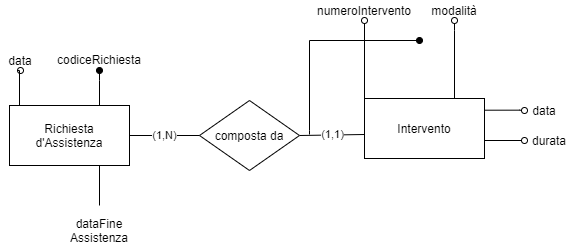
\includegraphics[width=\linewidth]{image/entita_debole.png}
		\caption{Entità debole}
		\label{fig:enita_debole}
	\end{minipage}
\end{figure}
\paragraph{Figura 3}
lo schema mette in evidenza la presenza di una generalizzazione esclusiva totale tra le entità Persona Giuridica e Singolo Cittadino che differiscono per codice identificativo univoco. Una Persona Giuridica viene distinta tramite Partita Iva, mentre un Singolo Cittadino dal proprio CodiceFiscale.
L'entità Cliente mi rappresenta il sovrainsieme a cui facciamo riferimento. Esso viene poi classificato attraverso l'utilizzo di due specializzazioni, individuando così i suoi sottoinsiemi, ovvero tutti gli elementi che compongono l'insieme stesso. \\
		Con la prima generalizzazione totale indichiamo che un Cliente deve essere una Persona Giuridica \textbf{o} un Singolo Cittadino (quindi persona fisica). Questa netta distinzione è data dalla totalità (indicata dalla freccia nera), partizionando l'insieme in due sottoinsiemi.\\
		Analogo discorso viene fatto con la Persona Giuridica, specializzandola in Azienda ed Ente Pubblico.\\
		Inoltre, entrambe le specializzazioni sono DISGIUNTE perché non può succedere che una persona giuridica sia allo stesso tempo una persona fisica.\\
		Un caso critico che si può presentare a causa della sua forma (gerarchie di specializzazione) riguarda l'ereditarietà multipla. Questo problema però non viene riscontrato in questo tipo di schema in quanto non abbiamo entità che appartengono a più gerarchie di specializzazione.\\
		Infine, è importante notare come tutte le entità ereditino gli attributi da cui derivano, più in particolare tutti gli attributi di Cliente verranno ereditati da qualsiasi entità appartenente a questa porzione di schema e le entità Azienda ed Ente Pubblico vengono individuate univocamente dagli attributi derivanti da Persona Giuridica.\\
\paragraph{Figura 4} 
lo schema mette in evidenza la presenza di un'entità debole che necessita della presenza di una richiesta d'assistenza per poter essere distinta univocamente.
Prima cosa da notare è la scelta di un attributo opzionale (dataFineAssistenza) in quanto esso verrà aggiunto una volta terminato l'ultimo intervento.
		Inoltre, la relazione \textit{"composta da"} è una relazione \textbf{molti a uno} perché una Richiesta di Assistenza può essere composta da molti interventi, mentre un intervento 
		appartiene ad una sola specifica richiesta.\\
		
\begin{figure}[!ht]
	\centering
	\begin{minipage}[b]{0.4\textwidth}
		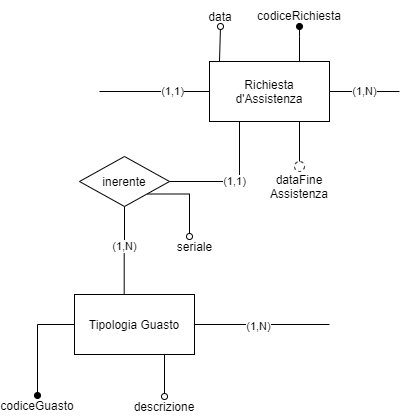
\includegraphics[width=\linewidth]{image/assistGuasto.png}
		\caption{Richiesta d'Assistenza inerente ad una tipologia di guasto}
		\label{fig:RichiestaInerenteGuasto}
	\end{minipage}
	\hfill
	
\end{figure}
\paragraph{Figura 5}
in questa figura si nota la modellazione della relazione tra Richiesta d'Assistenza e Tipologia Guasto:\\
E' stato deciso di collegare alla Richiesta d'Assistenza un seriale, cioè il numero di serie del sistema per il quale si vuole essere assistiti; non necessariamente a quest'ultimo deve far riferimento un sistema specifico, siccome ciò a cui siamo interessati è il tipo di guasto presente.\\
Sarà compito di un livello di astrazione superiore il controllo dell'autenticità della Richiesta d'Assistenza.\\ 
\subsection{Regole di derivazione}
Le regole di deriavazione sono delle informazioni ottenute tramite concetti dello schema, oppure mediante delle deduzioni. Nel modello concettuale analizzato è presente un attributo derivato, 
che permette ad ogni Tecnico di salvare il numero di ore lavorate mensilmente.\\
Questo permette di non dover scansionare tutti gli Interventi presenti nella base di dati per ricavare l'informazione.
L'attributo \textbf{Tecnico->oreLavorateMensilmente} sarà quindi aggiornato ogni volta che un Tecnico verrà assegnato ad un Intervento.\\
E' possibile calcolarlo sommando tutti i valori di \textbf{Intervento->durata} che si riferiscono al Tecnico in questione e al mese corrente.\\
Ogni volta che il mese finisce deve essere azzerato.\\

\subsection{Vincoli d'integrità}
I vincoli d'integrità sono tutte le proprietà di una base-di-dati, sono esprimibili 
tramite dei predicati; questi devono essere veri per garantire la validità dello schema.\\
\newline
Di seguito sono riportati i vincoli d'integrità presenti nel modello E-R:
\begin{itemize}
	\item L'attributo  \textbf{Richiesta d'Assistenza->dataFineAssistenza} deve essere maggiore o uguale\\
	alla proprietà \textbf{Richiesta d'Assistenza->data}
	\item Se   \textbf{Richiesta d'Assistenza->dataFineAssistenza} non è \textbf{NULL} allora: il numero di Interventi appartenenti ad un'Assistenza deve essere minore o uguale alla differenza (in giorni) tra \\  \textbf{Richiesta d'Assistenza->data} e   \textbf{Richiesta d'Assistenza->dataFineAssistenza}.\\Questo vincolo deriva dal fatto che è possibile fare un Intervento al giorno per singola Richiesta d'Assistenza.
	\item L'attributo  \textbf{Intervento->durata} deve essere un valore nel dominio (0, 24).
	Il valore della durata è rappresentato tramite il sistema orario a 24 ore.
	\item Un Tecnico non deve essere assegnato a degli Interventi diversi nello stesso giorno.
	\item Un Tecnico non deve essere assegnato a degli Interventi facenti parte di una Richiesta d'Assistenza, relativa ad una determinata Tipologia di Guasto, da lui non risolvibili.
	\item L'attributo  \textbf{Tecnico->oreLavorateMensilmente} deve essere uguale alla somma di tutti i valori di  \textbf{Intervento->durata} a cui un Tecnico ha lavorato nel mese corrente.

	
\end{itemize}

\subsection{Pattern di progettazione}
I pattern di progetto sono delle soluzioni progettuali a problemi comuni. Si elencano di seguito i pattern più utilizzati nella progettazione concettuale in basi di dati, applicati allo schema concettuale illustrato precedentemente:
\begin{itemize}
	\item Relazione "parte-di":\\
	- Un'assistenza è composta da diversi interventi

\end{itemize}
	

\newpage
\section{Progettazione logica}
\rule{\linewidth}{1.5pt}
\\ \\ \\
		Lo scopo della progettazione logica è di costruire uno schema relazionale che rappresenti in modo accurato, efficiente e soprattutto correttamente tutte le informazioni descritte da uno schema ER prodotto durante la fase precedente. \\
		Questo non è una semplice trasformazione da un modello ad un altro per due motivi:
		\begin{itemize}
			\item non tutti i costrutti del modello ER possono essere tradotti nel modello relazionale;
			\item lo schema deve essere ristrutturato in modo che l'esecuzione delle operazioni avvenga il più efficientemente possibile
		\end{itemize}
		Inoltre si controllano e governano le ridondanze. Infatti per analizzarle si usano: 
		\begin{itemize}
			\item i volumi dei dati;
			\item operazioni attese;
			\item frequenza delle operazioni;
		\end{itemize}
		\'E utile dividere questo tipo di progettazione in due semplici step:
		\begin{itemize}
			\item ristrutturazione dello schema ER, basato sull'ottimizzazione e semplificazione dello schema;
			\item traduzione nel modello logico.
		\end{itemize}
		\begin{figure}[ht]
			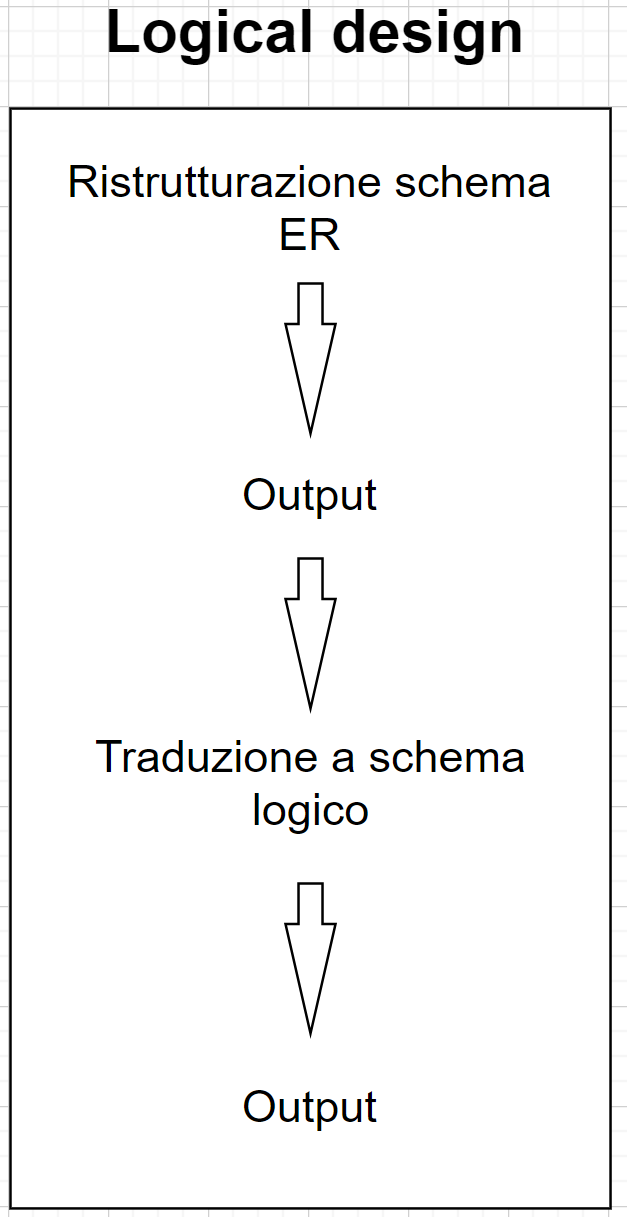
\includegraphics[width=4cm]{../Parata/Schema Prog. Logica}
		\end{figure}
	\subsection{Tabella dei volumi}
		In questa sezione andiamo a definire il numero di occorrenze per ogni entità e relazione presente all'interno dello schema ER. Viene ipotizzato che i volumi facciano riferimento all'attività dopo i suoi dieci anni di vita.\\
		\newline
		\renewcommand\arraystretch{2}
		\begin{tabular}{ |p{5cm}|p{2cm}|p{5cm}| }
			\hline
			\multicolumn{3}{|c|}{\textbf{Tabella dei volumi}} \\
			\hline
			\textbf{Entità/Relazione} & \textbf{Tipo} & \textbf{Volume} \\
			\hline
			Azienda & E & 3500 \\ \hline
			Ente Pubblico & E & 1500 \\ \hline
			Persona Giuridica & E & 5000 \\ \hline
			Singolo Cittadino & E & 5000 \\ \hline
			Cliente & E & 10000 \\ \hline
			effettua & R & 200000 \\ \hline
			Richiesta d'Assistenza & E & 200000 \\ \hline
			inerente & R & 200000 \\ \hline
			Tipologia Guasto & E & 30 \\ \hline
			composto da & R & 600000 \\ \hline
			Intervento & E & 600000 \\ \hline
			gestito da & R & 600000 \\ \hline
			è capace di risolvere & R & 750 \\ \hline
			Tecnico & E & 75 \\ \hline
		\end{tabular}

	
	\subsection{Tabella delle operazioni}
	Per ogni operazione indicata precedentemente, andiamo a definire la frequenza con la quale essa viene eseguita e la sua tipologia:
	\begin{itemize}
		\item \textbf{Batch}: operazioni che si possono "ignorare", ovvero vengono svolte quando il sistema non lavora in pieno regime (ad esempio tarda sera). Facendo così, si lascia spazio alle operazioni più importanti;\\
\textbf{Utilizzeremo una " B "}.
		\item \textbf{Interactive}: operazioni più importanti, dove la velocità di esecuzione deve essere veloce. Il tempo di risposta quindi deve essere veloce.\\
\textbf{Utilizzeremo una " I "}.
	\end{itemize}
		\renewcommand\arraystretch{2}
		\begin{tabular}{ |p{5cm}|p{2cm}|p{5cm}| }
			\hline
			\multicolumn{3}{|c|}{\textbf{Tabella delle operazioni}} \\
			\hline
			\textbf{Operazione} & \textbf{Tipo} & \textbf{Frequenza} \\
			\hline
			Operazione 1 & I &  19 volte a settimana \\ \hline
			Operazione 2 & I & 150 volte a settimana \\ \hline
			Operazione 3 & I & 450 a settimana \\ \hline
			Operazione 4 & B & 6 volte all'anno \\ \hline
			Operazione 5 & I & 30 volte a settimana \\ \hline
			Operazione 6 & B & 1 al giorno\\ \hline
			Operazione 7 & B & 1 volta all'anno \\ \hline
			Operazione 8 & I & 10 volte al giorno \\ \hline
			Operazione 9 & B & 1 volta a settimana \\ \hline
	
		
		\end{tabular}	

\subsection{Carico applicativo}
E' necessario calcolare il carico applicativo per scegliere tra le varie tipologie di traduzione quale adottare. Esso viene calcolato ed analizzato mediante la tabella dei volumi e la tabella delle operazioni.

\subsubsection{Tabella dei volumi}
\subsubsection{Tabella delle operazioni}


\subsection{Analisi delle ridondanze}
Nello schema ER è presente una singola ridondanza nell'entità Tecnico. Le ridondanze risultano essere utili perché possono essere informazioni più efficienti da ricavare direttamente invece che utilizzare apposite query per la loro determinazione. Essendo quindi derivabili, bisogna tenere aggiornata questa informazione.\\
	Per tenere una ridondanza presente all'interno dello schema, dobbiamo analizzare tutti i costi relativi ad esso e confrontarli con quelli che si ottengono qualora si ottenesse quella informazione in modo derivato.
	
	\subsubsection{Tabella dei volumi}
	Analizziamo tutte le componenti che si interfacciano con la ridondanza: \\ \newline
	\medskip
	\renewcommand\arraystretch{1,5}
	\begin{tabular}{|p{4cm}|p{4cm}|p{4cm}|}
		\hline
		\multicolumn{3}{|c|}{\textbf{Elementi coinvolti}}\\
		\hline
		Tecnico & \centering{E} & 75\\
		\hline
		gestito da & \centering{R} & 600.000\\
		\hline
		Intervento & \centering{E} & 600.000\\
		\hline
	\end{tabular}
	
	\subsubsection{Tabella delle operazioni}	
	Analizziamo tutte le operazioni che agiscono direttamente con la ridondanza: \\ \newline
	\medskip
	\renewcommand\arraystretch{1,5}
	\begin{tabular}{|p{4cm}|p{4cm}|p{4cm}|}
		\hline
		\multicolumn{3}{|c|}{\textbf{Operazioni coinvolte}}\\
		\hline
		Operazione 3 & I & 450 a settimana\\
		\hline
		Operazione 6 & B & 1 al giorno\\
		\hline
	\end{tabular}

	\subsubsection{Tabella degli accessi in riferimento all'operazione 3}
	Il costo di una operazione (calcolato usando una tabella dei volumi) e lo schema di navigazione possono essere riassunti nella tabella degli accessi: \\ \newline
	\begin{tabular}{|p{4cm}|p{4cm}|p{4cm}|p{4cm}|}
		\hline
		\multicolumn{4}{|c|}{\textbf{Tabella degli accessi senza la presenza di ridondanza}}\\
		\hline
		Concept & Type & Accesses & Type \\
		\hline
		Tecnico & E & 1 & R \\
		\hline
		gestito da & R & 1 & R \\ 
		\hline
		Intervento & E & 1 & W \\
		\hline
	\end{tabular} \\
	\newline
	\textbf{Analizziamo ora i costi:}
	\begin{itemize}
		\item 75 * 2 = 150 (costi in riferimento all'accesso a Tecnico e gestito da)
		\item 75 * 2 = 150 (costi in riferimento alla scrittura in Intervento)
		\item 150 + 150 = 300 (costo totale giornaliero dell'operazione)
	\end{itemize}
	\begin{tabular}{|p{4cm}|p{4cm}|p{4cm}|p{4cm}|}
		\hline
		\multicolumn{4}{|c|}{\textbf{Tabella degli accessi con la presenza di ridondanza}}\\
		\hline
		Concept & Type & Accesses & Type \\
		\hline
		Tecnico & E & 1 & W \\
		\hline
		gestito da & R & 1 & R \\ 
		\hline
		Intervento & E & 1 & W \\
		\hline
	\end{tabular} \\
	\newline
	\textbf{Analizziamo ora i costi:}
	\begin{itemize}
		\item 75 * 2 = 150 (costi in riferimento ala modifica di Tecnico)
		\item 75 (costi in riferimento alla relazione gestito da)
		\item 75 * 2 = 150 (costi in riferimento alla scrittura in Intervento)
		\item 150 + 75 + 150 = 375 (costo totale giornaliero dell'operazione)
	\end{itemize}
	
	Come possiamo notare, il costo con la presenza di ridondanza è leggermente maggiore (esattamente del 25\%), ma come vedremo nella prossima operazione, questo ci comporterà un beneficio.
	
	\subsubsection{Tabella degli accessi in riferimento all'operazione 6}
	Il costo di una operazione (calcolato usando una tabella dei volumi) e lo schema di navigazione possono essere riassunti nella tabella degli accessi: \\ 
	\newline
	\medskip
	\renewcommand\arraystretch{1,5}
	\begin{tabular}{|p{4cm}|p{4cm}|p{4cm}|p{4cm}|}
		\hline
		\multicolumn{4}{|c|}{\textbf{Tabella degli accessi in presenza di ridondanza}}\\
		\hline
		Concept & Type & Accesses & Type \\
		\hline
		Tecnico & E & 1 & R \\
		\hline
	\end{tabular}\\
	\newline
	Tenendo in considerazione che il costo di una operazione di read è uguale ad un accesso, con la presenza della ridondanza, ottenere l'informazione derivabile (Tecnico->oreLavorateMensilmente) ci viene a costare esattamente 75 accessi al giorno cioè:
	\begin{itemize}
		\item 75 * 1 = 75 accessi giornalieri
		\item 75 * 26 = 1950 accessi totali mensili
	\end{itemize}
	\begin{tabular}{|p{4cm}|p{4cm}|p{4cm}|p{4cm}|}
		\hline
		\multicolumn{4}{|c|}{\textbf{Tabella degli accessi senza la presenza di ridondanza}}\\
		\hline
		Concept & Type & Accesses & Type \\
		\hline
		Tecnico & E & 1 & R \\
		\hline
		gestito da & R & 1 & R \\ 
		\hline
		Intervento & E & 1 & R \\
		\hline
	\end{tabular} \\
	\newline
	Senza la presenza della ridondanza, è necessario:
	\begin{itemize}
		\item 75 * 3 = 225 accessi al giorno
		\item 225 * 26 = 5850 accessi mensili
	\end{itemize}
	\textbf{Conclusioni:}
	\begin{itemize}
		\item dall'analisi svolta, vediamo come la presenza della ridondanza risulti conveniente in quanto il numero di accessi è inferiore del 67\%
		\item inoltre, c'è da tenere in considerazione che ogni volta che si effettua l'accesso alla tabella degli Interventi, bisogna filtrare 600.000 righe
	\end{itemize}
	

\subsection{Rimozione delle generalizzazioni}
Per tradurre lo schema E-R bisogna rimuovere le varie generalizzazioni:\\
\newline
\textbf{Accorpamento dei figli della generalizzazione nel genitore}
\begin{itemize}
	\item Le entità Azienda e Ente Pubblico vengono eliminate e le loro proprietà vengono aggiunte a Persona Giuridica. Per distinguerli viene aggiunto l'attributo \textbf{tipo}. \\Il suo valore è un carattere che assume \textbf{A} oppure \textbf{E}, in cui il primo indica azienda ed il secondo ente pubblico.\\
	Si effettua questo accorpamento perché le attività svolte sono identiche. \\La superchiave \textbf{partitaIva} è la medesima, perciò non distinguibili senza la presenza della tipologia.
	\item Le entità Persona Giuridica e Singolo Cittadino vengono eliminate e le loro proprietà vengono aggiunte a Cliente. \\Per distinguerle viene utilizzato come superchiave un unico attributo denominato \textbf{codiceFiscale/partitaIva}, con valore rispettante le caratteristiche di un reale numero di Partita Iva, nel caso in cui si tratta di una persona giuridica, e quelle di un reale Codice Fiscale nel caso in cui si tratta di un singolo cittadino.\\ L'attributo \textbf{tipo} di Persona Giuridica diventa opzionale a seconda della tipologia della superchiave.\\
	Si effettua questo accorpamento perché le attività svolte sono identiche.
\end{itemize}

%\subsection{Partizionamento /accorpamento}

\subsection{Regole di derivazione}
\textbf{Tecnico->oreLavorateMensilmente:} attributo derivato che contiene la somma delle ore che un Tecnico ha lavorato nel mese corrente ed è un valore che deve essere maggiore o uguale a zero.\\
Vale sempre che: 
\begin{itemize}
	\item  0 <= \textbf{Tecnico->oreLavorateMensilmente}
		\begin{itemize}\item sarà zero nel momento in cui il Tecnico non ha ancora lavorate nel mese corrente\end{itemize}
	\item Somma(\textbf{Intervento->durata} inerente al tecnico interessato) = \textbf{Tecnico->oreLavorateMensilmente}
		\begin{itemize}
		\item verrà aggiornato ogni volta che viene aggiunto un Intervento a qui un Tecnico lavorerà
		\end{itemize}
\end{itemize}
\subsection{Vincoli d'integrità}
	\begin{enumerate}
	\item Nel ciclo tra [Richiesta d'Assistenza, Intervento, Tecnico, Tipologia Guasto]
		\begin{itemize}
		\item Un Tecnico non deve essere assegnato ad un Intervento che fa riferimento ad una Richiesta d'Assistenza inerente ad una Tipologia Guasto che quel determinato tecnico non sa risolvere
		\end{itemize}
	\item Dopo che ho asseganto un valore all'attibuto \textbf{Richiesta d'Assistenza->dataFineAssistenza} non possono esistere degli Interventi inerenti a quella Richiesta che hanno l'attributo\\
\textbf{Intervento->data} maggiore di \textbf{Richiesta d'Assistenza->dataFineAssistenza}
\end{enumerate}

\subsection{Vincoli d'integrità aggiuntivi dello schema E-R ristrutturato}
\begin{figure}[h]
	\centering
	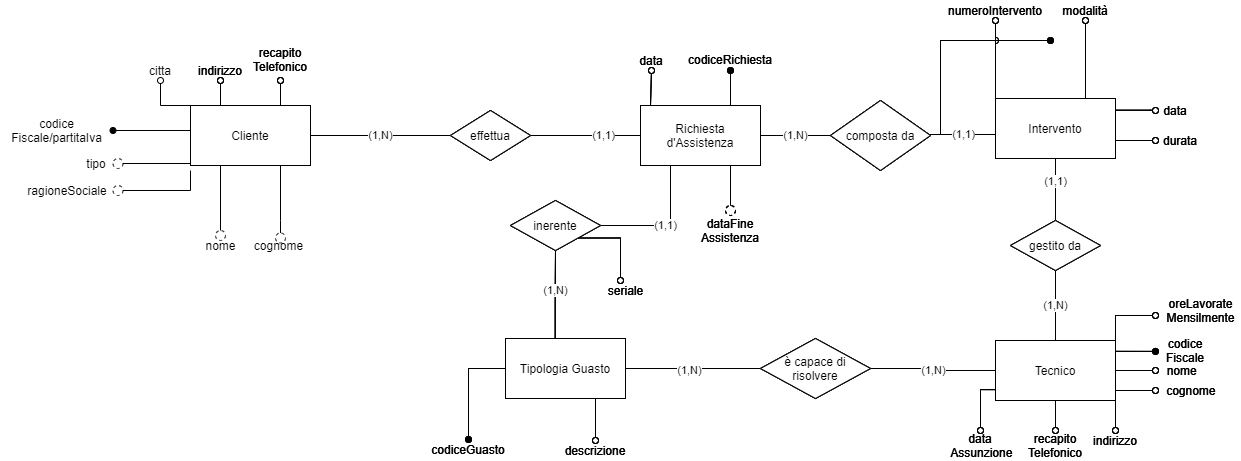
\includegraphics[width=0.9\linewidth]{image/er_ristrutturato}
	\caption{}
	\label{fig:erristrutturato}
\end{figure}


\subsection{Modello relazionale}
\begin{tabular}{|p{\textwidth}|}
	\hline
	{\cellcolor[HTML]{a3cbf8}{\color[HTML]{000000} \textbf{Cliente}}}
	\\
	\hline
	\\                       
	Cliente(\underline{codiceFiscale/partitaIva},indirizzo,citta,recapitoTelefonico,ragioneSociale,\\codiceFiscaleReferente,nome,cognome, tipo) \newline  \\               
	Unique--\textgreater codiceFiscaleReferente
	\\
	NotNull--\textgreater indirizzo,citta, recapitoTelefonico
	\\
	\\
	\hline
\end{tabular}
\\ \\ \\
\begin{tabular}{|p{\textwidth}|}
	\hline
	{\cellcolor[HTML]{a3cbf8}{\color[HTML]{000000} \textbf{Richiesta d'Assistenza}}}
	\\
	\hline  
	\\               
	Richiesta d'Assistenza(\underline{codiceRichiesta},data,dataFineAssistenza,\textit{codiceCliente*},\textit{codiceGuasto*}, seriale) \\               
	NotNull--\textgreater data, seriale \\ 
	codiceCliente FK--\textgreater Cliente.partitaIva/codiceFiscale \\
	codiceGuasto FK--\textgreater TipologiaGuasto.codiceGuasto
	\\
	\\
	\hline
\end{tabular}
\\ \\ \\
\begin{tabular}{|p{\textwidth}|}
	\hline
	{\cellcolor[HTML]{a3cbf8}{\color[HTML]{000000} \textbf{Intervento}}}
	\\
	\hline
	\\                       
	Intervento(\underline{codiceRichiesta},\underline{numeroIntervento},modalità,data,durata,\textit{cfTecnico*}
	\\               
	NotNull--\textgreater modalità,data,durata
	\\
	cfTecnico FK--\textgreater Tecnico.codiceFiscale
	\\ \\
	\hline
\end{tabular}
\\ \\ \\
\begin{tabular}{|p{\textwidth}|}
	\hline
	{\cellcolor[HTML]{a3cbf8}{\color[HTML]{000000} \textbf{Tecnico}}}
	\\
	\hline
	\\                       
	Tecnico(\underline{codiceFiscale},nome,cognome,indirizzo,recapitoTelefonico,dataAssunione,\\oreLavorateMensilmente)
	\\               
	NotNull--\textgreater nome,cognome,indirizzo,recapitoTelefonico,dataAssunione,oreLavorateMensilmente
	\\
	cfTecnico FK--\textgreater Tecnico.codiceFiscale
	\\ \\
	\hline
\end{tabular}
\\ \\ \\
\begin{tabular}{|p{\textwidth}|}
	\hline
	{\cellcolor[HTML]{a3cbf8}{\color[HTML]{000000} \textbf{è capace di risolvere}}}
	\\
	\hline
	\\                       
	è capace di risolvere(\underline{codiceFiscale},\underline{codiceGuasto}
	\\ \\
	\hline
\end{tabular}
\\ \\ \\
\begin{tabular}{|p{\textwidth}|}
	\hline
	{\cellcolor[HTML]{a3cbf8}{\color[HTML]{000000} \textbf{Tipologia Guasto}}}
	\\
	\hline
	\\                       
	Tipologia Guasto(\underline{codiceGuasto},descrizione) 
	\\               
	NotNull--\textgreater descrizione
	\\
	\\
	\hline
\end{tabular}

\subsection{Regole di derivazione}

\subsection{Vincoli d'integrità}

\subsection{Vincoli d'integrità aggiuntivi del modello relazionale}

\subsection{Normalizzazione}
\subsubsection{Prima forma normale(1FN)}
	Per vedere se è in Prima Forma Normale, dobbiamo semplicemente controllare che tutti gli attributi dello schema abbiano domini "atomici", ovvero che non siano composti o multivalore. \\
	E' questo il caso.
\subsubsection{Seconda forma normale(2FN)}
	Il modello logico relazionale è in Seconda Forma Normale perché ogni attributo non-primo, cioè non appartenente a nessuna chiave, dipende completamente da ogni chiave (ovvero non dipende solamente da una parte di chiave).
\subsubsection{Terza forma normale(3FN)}
	Il modello risulta essere in Terza Forma Normale in quanto, per ogni dipendenza funzionale (non banale) Y-->Z definita su di esso, Y è una superchiave oppure ogni attributo in Z è primo, cioè contenuto in almeno una chiave del modello.
\newpage
\section{Progettazione fisica}
\rule{\linewidth}{1.5pt}
\subsection{Data Definition Language (DDL)}
	Nell'SQL, la definizione dei dati o DDL è una sintassi per creare e modificare oggetti nel database come tabelle, indici e utenti. Esso è legato alla creazione del dizionario dei dati e l'eventuale definizione delle strutture di memorizzazione e dei metodi di accesso ai dati e rappresenta il primo passo della progettazione fisica.	\\
	Di seguito elencheremo tutti strutture ottenute tramite DDL:
	
	\subsubsection{Clienti}
		\begin{figure}[h]
			\centering
			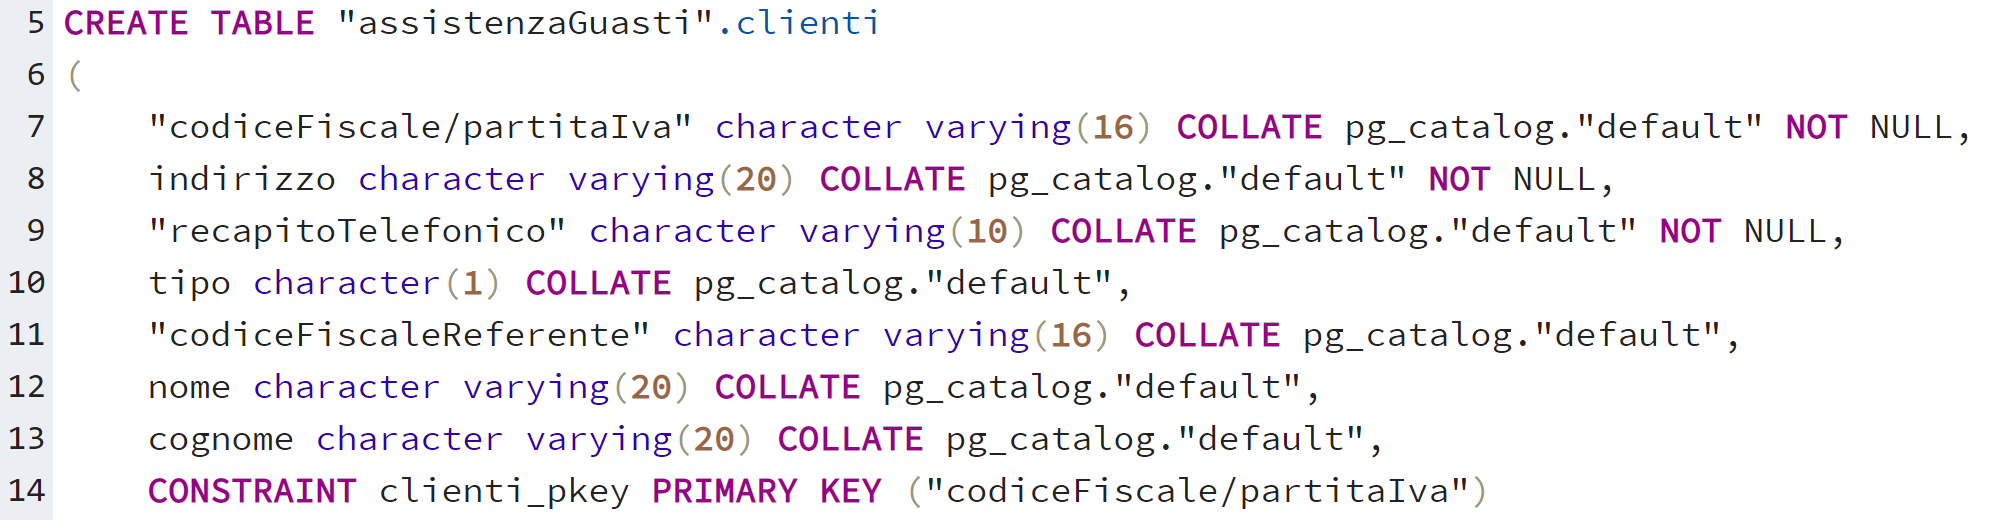
\includegraphics[width=0.9\linewidth]{Immagini SQL/Clienti}
			\caption{Definizione tabella Clienti in SQL}
			\label{clientisql}
		\end{figure}
		Di seguito viene effettuata un'analisi del codice. \\
		
\subsection{Indici}
\subsubsection{Indici implementati}
\subsection{UDF}
\subsection{Operazioni}
\subsubsection{Operazione 1: inserisci cliente}
\subsection{Trigger}
\subsubsection{Evento 1}
\subsection{Pulizia}
\subsubsection{Implementazione}
\newpage

\section{Implementazione}
\rule{\linewidth}{1.5pt}
\subsection{Hardware e Tecnologie Utilizzate}
Per testare e condividre il database a tutti i membri abbiamo creato un server utilizzando un \textbf{Raspberry Pi 3} con all'interno \textbf{Raspbian}.
\begin{itemize}
	\item CPU: Arm Cortex-A7
	\item RAM: 1GB
\end{itemize}
Dopo aver installato il sistema operativo abbiamo potuto interfacciarci tramite \textbf{openssh-server}.\\
A questo punto abbiamo installato \textbf{postgresql-11} seguendo le istruzioni riportate dalla guida ufficiale.
\begin{itemize}
	\item Installazione: https://www.postgresql.org/download/linux/ubuntu/
\end{itemize}
Abbiamo quindi a disposizione la console di postgres che ci permette di eseguire le query simile all'interazione \textbf{tty}; abbiamo quindi deciso di permettere a postgres di accettare le connessioni
da parte di client \textbf{pgAdmin4}.\newline
Per farlo c'è bisogno di modificare i file di conficurazioni iniziale di postgresql; nel nostro caso si trovano in \\ \textbf{/etc/postgresql/11/main},
più precisamente dobbiamo modificare i file:
\begin{itemize}
	\item \textbf{pg\_hba.conf}: Nello specifico va inserita un riga che specifica quali sono gli indirizzi IP di cui postgres può fidarsi.
	\item \textbf{postgresql.conf}: Nello specifico va aggunta la riga \textbf{listen\_addresses = '*'}.
\end{itemize}
E' importante sottolineare che: \underline{!QUESTE IMPOSTAZIONI DEL SERVER SERVONO A FAR SI CHE}\\ 
\underline{L'ACCESSO E IL TESTING SIA PIU' VOLCE, NON E' PER NULLA SICURO USARE QUESTE}\\
\underline{IMPOSTAZIONI IN UN PRODOTTO FINALE!}
\subsection{Popolazione della base di dati}
\subsection{Connessione alla base di dati}
\subsection{Preparazione iniziale}
\subsection{Cliente}

...

\subsection{Disconnessione dalla base dei dati}
\newpage
\section{Analisi dei dati}
\rule{\linewidth}{1.5pt}

\newpage

\section{Bibliografia}
\rule{\linewidth}{1.5pt}





\end{document}
